\chapter{Concept}\chaplabel{3}

This chapter aims to identify a promising approach to address the task. A thorough analysis of the challenges associated with the task is conducted first. This analysis serves as a foundation for comparing and contrasting different methods and algorithms to determine the most effective approach.

\section{Task Challenges}

This study is confined to a particular building on the THL campus, and concentrates on a single facade. As a result, the roller shutters installed on this particular building are relatively homogeneous in terms of their features, such as texture, brands, and colors. Additionally, the images used for analysis are static, and do not require real-time processing. Despite these factors, the realization of the proposed detection method may face several challenges. Three main challenges are identified and discussed in the following sections.

\subsection{Round-the-clock detection}

Detecting objects reliably under different weather conditions and at different times of day poses a challenge. Changes in light intensity and color temperature can significantly affect the appearance features of roller shutters, while camera's performance may also degrade due to factors such as lighting and noise, thereby affecting the image quality. Figure \ref{fig:8} depicts how the image of the same window would differ under various conditions. 

\begin{figure}[h]
  \centering
  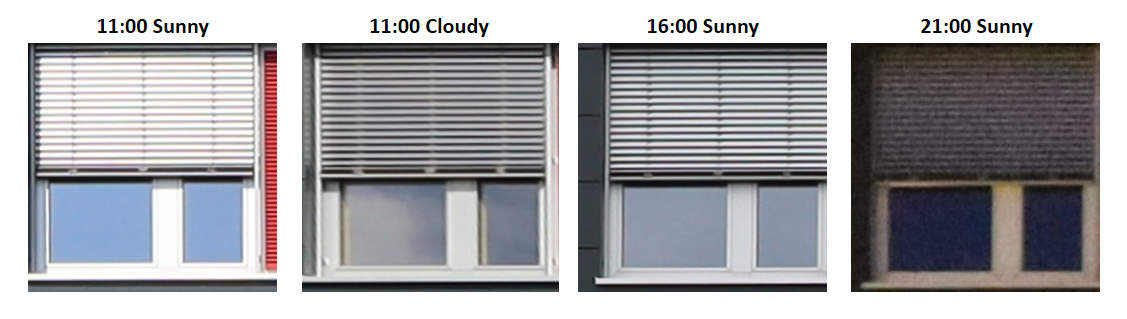
\includegraphics[width=1\textwidth]{Figures/round-the-clock.png}
  \caption{Images of the same window taken at different time or under different weather conditions}
  \label{fig:8}  
\end{figure}

\subsection{Impact of occlusion}

Occlusion is considered a existing and challenging issue in machine vision applications that can significantly hinder feature extraction and classification when the target is obscured. The problem is further exacerbated in the current study, where not only the roller shutter need to be detected, but its degree of closure must also be calculated. Figure \ref{fig:9} describes examples of occlusion scenarios in this task. Addressing this challenge requires a highly demanding solution to mitigate the impact of occlusion.

\begin{figure}[h]
  \centering
  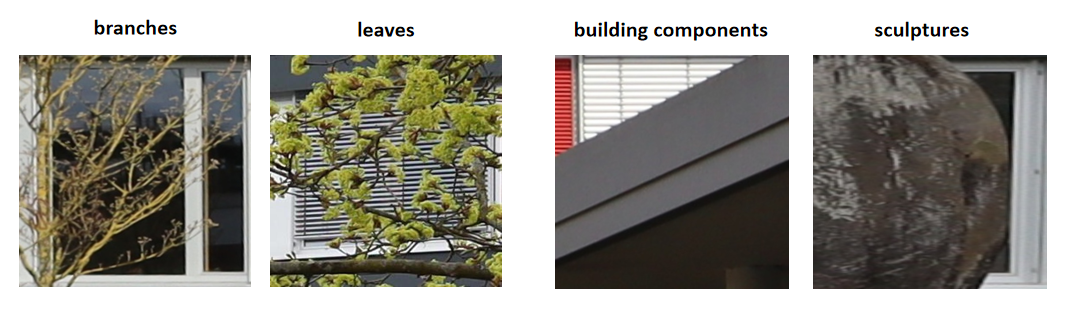
\includegraphics[width=1\textwidth]{Figures/occlusion examples.png}
  \caption{Images of various occlusion scenarios}
  \label{fig:9}  
\end{figure}

\subsection{Measurement of the Degree of Closure (DoC)}

In order to accurately determine the percentage of how much a roller shutter is lowered (In this bachelor thesis, DoC is used to represent such percentage) , a reliable and consistent measurement method that can be applied to all situations is necessary. While the length and area of a window remain fixed in the real world, the shape of the window in the 2D world of digital photography can be affected by the camera angle, making it challenging to obtain clear and upright images for accurate measurements. Additionally, distinguishing the boundary between the window and the roller shutter may also pose difficulties.

\section{Evaluation of Methods}

In chapter 2, three promising methods were introduced, which are:

\begin{enumerate}
  \item traditional digital signal processing techniques like template matching
  \item traditional machine learning with classification and regression
  \item deep learning with object detection and segmentation
\end{enumerate}

Based on their performance for addressing the challenges mentioned above, one method will be selected for use in this study. This section presents an analysis of the strengths and limitations of each method. In order to ensure simplicity throughout this section, this bachelor thesis employs \textbf{DSP Method, TML Method} and \textbf{DL Method}, respectively, to represent these methods. Table \ref{tab:1} provides an overview of the performance of the three methods in addressing the challenges posed by the task, which would be explained in the following paragraphs.

\begin{table}
  \centering
  \caption{Evaluation of Three Methods}
  \label{tab:1}
  \begin{tabular}{cccc}
    \toprule
    Methods & Round-the-clock Detection & Occlusion & Measurement \\
    \midrule
    DSP Method &  + & - & + \\
    TML Method & ++ & + & + \\
    DL Method & +++ & ++ & ++ \\
    \bottomrule
  \end{tabular}
  \vspace{0.8em}
  \begin{tablenotes}
    \item \textbf{Note:} The more plus signs (+) indicate better performance, while the minus sign (-) indicates the method is not suitable for addressing the challenge.
    
  \end{tablenotes}
\end{table}

The first challenge is round-the-clock detection, for which the DL method performs the best. DSP Method can be a fast and simple solution, but it requires several preprocessing steps to reduce the impact of lighting or noise. However, these steps should be designed carefully while adaptive processing steps may hinder the accuracy of detection to a great extent. The TML method has the advantage of being able to classify or regress new and unknown patterns or scenarios by learning the statistical patterns of the data, thus having stronger generalization ability. However, it still requires manual feature engineering, which demands specific knowledge and experience. On the other hand, DL method may require some time to train the model, but it can overcome the limitations of the other two methods. By learning large amounts of data, DL can automatically extract features and better generalize to new data. Since the speed of detection and training time are not the primary requirements of this study, the DL method is considered the most appropriate for addressing round-the-clock detection issues.

The second challenge is occlusion. DL method still performs best in tackling this issue. DSP Method like template matching relies on comparing the raw pixel values of the input image to a pre-defined template, which is not robust to changes in the appearance of the object due to occlusion. The TML method can improve the robustness of the model by selecting features that are insensitive to occlusion, and the classifier design can use a combination of multiple classifiers to mitigate the effects of occlusion. However, for different occlusion cases, the features need to be manually selected and designed again, which makes the implementation and adjustment of the algorithm more cumbersome. The DL method provides a better solution with the help of data augmentation in the training process, and can automatically learn feature representations in images, enabling them to recognize objects even when they are partially occluded. DL models can also incorporate multiple scales and viewpoints of the object to improve recognition accuracy.

In terms of measuring the DoC, the shape of the roller shutter is rectangular, which matches the shape of a bounding box. Therefore, using bounding boxes as a representation is considered appropriate for this study. Although all three methods can provide bounding boxes to locate the target, the DL method can provide more detailed and accurate bounding boxes, as well as other information such as the class and confidence level of the target. This additional information enables more comprehensive and precise object detection and recognition, using techniques such as Non-Maximum Suppression (NMS), which outputs only the bounding boxes with the highest confidence level in a certain region. If a pixel-level measurement of DoC is required, a deep learning segmentation task can generate a mask of the roller shutters to improve the measurement accuracy.

Overall, the superior performance of the DL method, which surpasses the other two methods in every aspect, makes it the preferred approach for this bachelor thesis.

\section{Evaluation of Algorithms}

In order to select the most efficient algorithm for the current task, it is crucial to evaluate the candidate deep learning algorithms. While both object detection and segmentation algorithms can achieve recognition, this bachelor thesis will only focus on algorithms primarily designed for object detection. This is because although segmentation can provide precise classification of every single pixel, it requires far more training to achieve the same level of accuracy as object detection. On the other hand, as is mentioned above, the use of rectangular bounding box would be enough for measurement. 

In the previous chapter, several one-stage and two-stage object detection algorithms were mentioned. This bachelor thesis includes R-CNN series, EfficientDet, YOLO series, RetinaNet, and SSD series as candidates for evaluation. To analyze the performance of these algorithms, two metrics were considered: Mean Average Precision (mAP) and Frames Per Second (FPS). While real-time detection was not a requirement for the task, higher FPS could indicate faster processing times when handling a large number of static images, and was therefore taken into consideration.

This bachelor's thesis compiled the test results of each algorithm's most complex model (which maximize the mAP at the cost of FPS) on the COCO dataset (test-dev2017), as shown in Table \ref{tab:2}. It can be seen that the later YOLO series achieved a generally higher mAP and faster detection speeds compared to the other algorithms. Among the YOLO series, YOLOv5 may be not the latest version of YOLO series, but it remains one of the state-of-art algorithms in the field of object detection and more researches are based on it than any other YOLO's later version. Therefore, this bachelor thesis chooses YOLOv5-v6.0 as the proposed algorithm to address the detection of roller shutter status.

\begin{table}
  \centering
  \caption{Performance on COCO Dataset}
  \label{tab:2}
  \begin{tabular}{cccccc}
    \toprule
    Algorithms & Proposal & Backbone & Size & FPS & mAP (\%) \\
    \midrule
    \midrule
    Faster R-CNN \cite{wang2019region} & 01/2016 & ResNet-50 & - & 9.4 & 59.2 \\
    R-FCN \cite{redmon} & 03/2016 & ResNet-101 & - & 12 & 51.9 \\
    FPN FRCN \cite{redmon} & 10/2017 & ResNet-101 & - & 6 & 59.1 \\
    \midrule
    RetinaNet \cite{lin2017focal} & 06/2018 & ResNet-101 & 800 & 5.1 & 57.5 \\
    \midrule
    EfficientDet-D3 \cite{tan2020efficientdet} & 03/2020 & Efficient-B3 & 896 & 23.8 & 65.0\\
    \midrule
    SSD \cite{liu2016ssd} & 12/2016 & VGG-16 & 512 & 22 & 48.5 \\
    SSD \cite{redmon} & 12/2016 & ResNet-101 & 513 & 8 & 50.4 \\
    DSSD \cite{redmon} & 07/2017 & ResNet-101 & 513 & 6 & 53.3 \\
    \midrule
    YOLOv3-SPP \cite{redmon2018yolov3} & 04/2018 & Darknet-53 & 608 & 20 & 60.6 \\
    YOLOv4 \cite{bochkovskiy2020yolov4} & 04/2020 & CSPDarknet-53 & 608 & 23 & 65.7 \\
    YOLOv5x \cite{ultralytics} & 05/2020 & CSPDarknet-53 & 640 & - & 68.9 \\
    YOLOv5x6 \cite{ultralytics} & 05/2020 & CSPDarknet-53 & 1280 & - & 72.7 \\
    \bottomrule
  \end{tabular}
  \vspace{0.8em}
  \begin{tablenotes}
    \item \textbf{Note:}  (-) indicates that the corresponding metrics were not found.
    
  \end{tablenotes}
\end{table}

\section{Addressing Challenges Using Bounding Boxes}

Now that object detection algorithm YOLOv5 is selected for this task, how it can solve the existing challenges need to be discussed before moving on to the implementation part. One of the main features of YOLOv5 and other object detection algorithm is using bounding boxes to localize the object. Although the performance of an algorithm can be decided by its architecture to a large extent, the ability to tackle specific challenges can be improved if the bounding boxes are used wisely and certain rules are set.

As the round-the-clock detection can be well realized through existing YOLOv5 network architecture and feature extraction strategies, this section focuses mainly on the newly proposed solutions for addressing occlusion and measurement of DoC in roller shutter detection.

\subsection{Solution for heavy occlusion}

Unlike the common goal of object detection algorithms, which is to recognize objects despite all kinds of occlusion, the goal of this task is not only to recognize but also to provide precise measurements. Therefore, we do not want the model to sacrifice the accuracy of measurements by predicting the possible area of the entire roller shutter in the presence of heavy occlusion. To address this, a balance is defined to split occlusion scenarios into two categories: \textbf{Mild occlusion}, which the model should be robust enough to “see through”, such as branches, leaves; \textbf{Heavy occlusion}, which should be exclude by the model, such as building components, sculptures, regardless of whether the part obscured is part of roller shutters. For heavy occlusion scenarios, this subsection will explain how a decision tree can be applied to tackle them.

To achieve this, the status of roller shutters are set as open, closed or blocked. This gives rise to another problem when we defining object classes. If we set shutter as the only object class, there will be only two different results based on whether roller shutters are detected or not. To be more specific, if roller shutter is not detected in the image, the status could either be open or blocked, which we cannot tell from each other based on the detection results. Therefore, this bachelor thesis add another object class to detect window glass, which can help determine the status.

As shown in Figure \ref{fig:10}, ten scenarios are used to simulate the roller shutter status in reality. In some scenarios, although strong occlusion exists in the images, it has no influence on the determination of roller shutter status. This is because we only need to find out the demarcation between roller shutters and glass to judge the DoC. Therefore, as long as such demarcation is clear, any occlusion would not be considered affecting the detection result. This also give rise to another method to calculate DoC, which will introduced later in this section.

\begin{figure}[h]
  \centering
 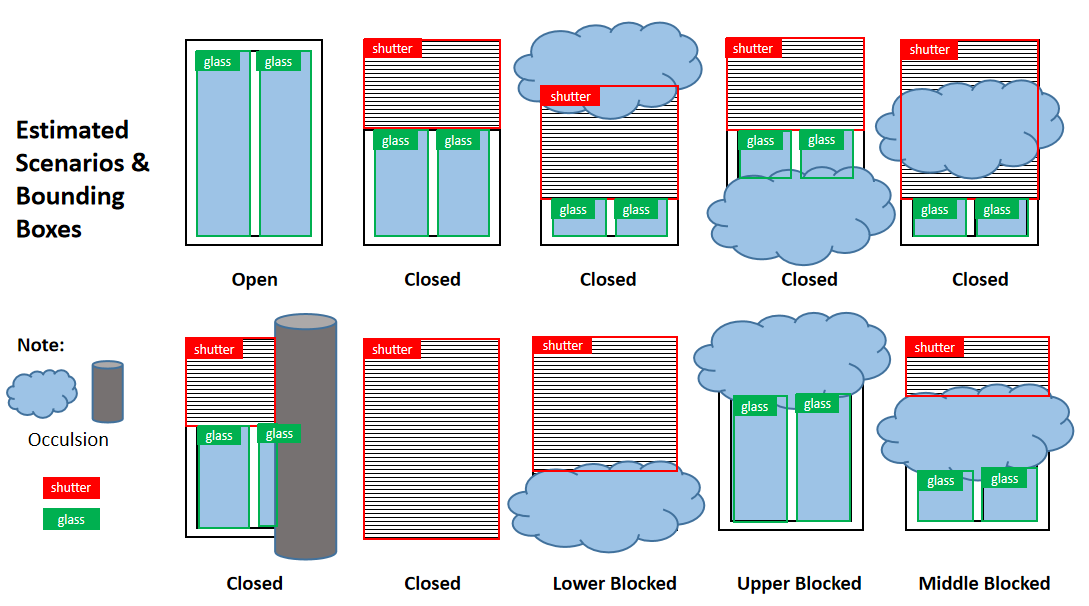
\includegraphics[width=1\textwidth]{Figures/Estimate BBs.png}
  \caption{Estimated Scenarios and Bounding Boxes with Two Object Classes "Shutter" and "Glass"
}
  \label{fig:10}
\end{figure}


\begin{figure}[h]
  \centering
 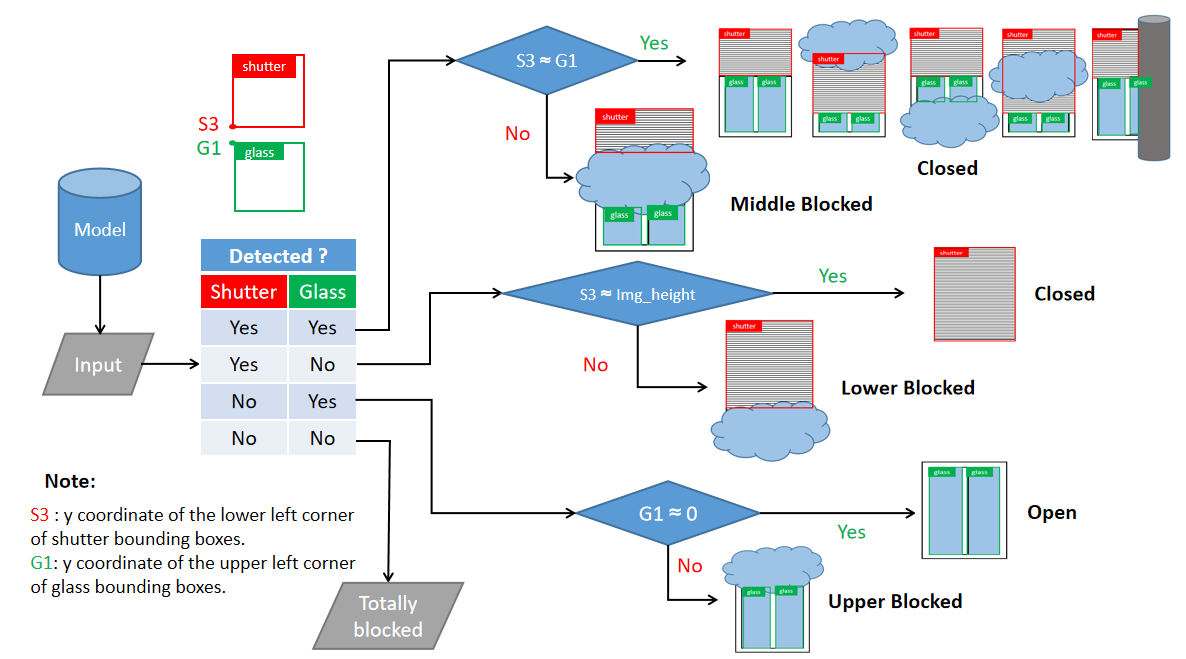
\includegraphics[width=1\textwidth]{Figures/Decision Tree.png}
  \caption{A Decision Tree to Determine The Roller Shutter Status
}
  \label{fig:11}
\end{figure}

To distinguish these scenarios by status, a decision tree is designed as figure \ref{fig:11} depicts, those scenarios can be split by simple logic comparing a few parameters of the bounding boxes. To be specific, \textbf{S3} and \textbf{G1}, which represent y coordinates of the lower left corner of shutter bounding boxes and the upper left corner of glass bounding boxes respectively. Those scenarios are split into four branches at first step based on the detection results:

\textbf{(1) Both the roller shutter and glass are detected.} This means the status is either closed or blocked. We need to examine whether the demarcation between the roller shutter and glass is clear by comparing G1 and S3. If G1 is approximately equal to S3, we can determine that the roller shutter status is closed. Otherwise, something is blocking the window in the middle, and the end of the roller shutter could be anywhere above G1 and below S3.

\textbf{(2) Only the roller shutter is detected.} In this case, we cannot tell whether the window glass is fully covered by the roller shutter or partly by occlusion. Therefore, we compare S3 with the height of the window, which is the height of the image in practice (images for detection contain only the window without any background). If S3 is approximately equal to the height of the image, the roller shutter is considered fully closed. If not, it is considered blocked, and the exact DoC cannot be determined.

\textbf{(3) Only the glass is detected.} With the absence of the roller shutter, we cannot simply say that the roller shutter is open. This is because the roller shutter may be covered by occlusion that covers the upper part of the image. To address this problem, we need to check the value of G1. If it approaches 0, which ensures that the upper parts of the image may not be the roller shutter, then we can determine the status as open. Otherwise, we cannot determine whether the area above G1 in the image is glass or roller shutter, which we mark as blocked.

\textbf{(4) Neither the roller shutter nor glass is detected.} This indicates a failure in detection, which could be due to the poor performance of the detection model or the window being completely blocked by occlusion. Assuming that the algorithm works well, we also mark this scenario as blocked.

By using this logic to determine the roller shutter status, the detection model should be robust enough to handle heavy occlusion. However, the logic is not yet clear enough to put into practice because when comparing two parameters, "approximately equal to" cannot be understand by computer. Specific thresholds need to be determined and adjusted during implementation. Also, for mild occlusion, some optimizations have also been made, which are described in the next chapter. 
\subsection{Measurement of DoC}

The most straightforward way to calculate DoC according to its definition is:

$$ DoC = \frac{\text{Area of the Bounding Box}}{\text{Area of Corresponding Window}} \times 100\%
$$

As mentioned in previous evaluation of methods, the measurement of DoC can be achieved using bounding boxes due to their similar shape to roller shutters. However, The area of the bounding box may not express the true area of the Roller shutter. This is because bounding boxes are upright rectangular with their sides either vertical or horizontal. The roller shutter in the image, on the other hand, may not be upright due to shooting angles. Therefore, before detection, the cropped image of each window needed to be set upright to ensure the edge of the roller shutter in the picture is parallel to the edge of the bounding box. In addition, as the width of roller shutter is equal to the width of window and the height of window can be replaced by the height of cropped image in practice, the formula can simplified as 

$$ DoC = \frac{\text{Height of the Bounding Box}}{\text{Height of Image}} \times 100\%
$$

However, the formula may be flawed in certain situations, as discussed in the previous subsection. Using the height of the bounding box may not be appropriate when dealing with occlusion problems, where the bounding box only represents the unobstructed part of the roller shutter. Therefore, as the y coordinate of the bounding box's upper boundary may be 0 in normal cases, the y coordinate of the lower boundary (S3) is used to represent the height of the roller shutter. The final optimized formula is described as: 

$$ DoC = \frac{\text{S3}}{\text{Height of Image}} \times 100\%
$$

Since the height of the image is fixed and depends solely on the input size of the model, there is only one variable in the formula mentioned above. This means that this measurement method may be more resistant to errors. However, the validity of this formula depends on the assumption that each image for detection is only filled with a complete window, without any offset or redundant background in the vertical direction. While this may pose a challenge for localizing windows, the benefits of reducing error rates and minimizing the number of object classes for detection make it a worthwhile trade-off.

\subsection{Fusion}

To obtain accurate results, fusion is another effective method to mitigate the impact of heavy occlusion. In this bachelor thesis, three cameras are set up to capture images of the same building facade from different angles. This allows us to determine the optimal angle that provides the best representation of the roller shutter status and DoC.

As shown in Figure \ref{fig:13}, we considered all 19 possible scenarios using three cameras and estimated the fusion results for both the roller shutter status and DoC. Our estimation was based on three pre-defined rules, as follows:

\begin{enumerate}
\item The status is considered "blocked" only when all camera angles produce "blocked" results.
\item If the final status is "blocked", the DoC range would describe the possible maximum and minimum values. If multiple cameras detect a "blocked" status, the range would be narrowed as much as possible.
\item If "open," "close," or both are detected, the final status is determined by majority rule. If the final status is "closed," the average of the non-zero DoC values would be taken as the final DoC.
\end{enumerate}

\begin{figure}[h]
  \centering
  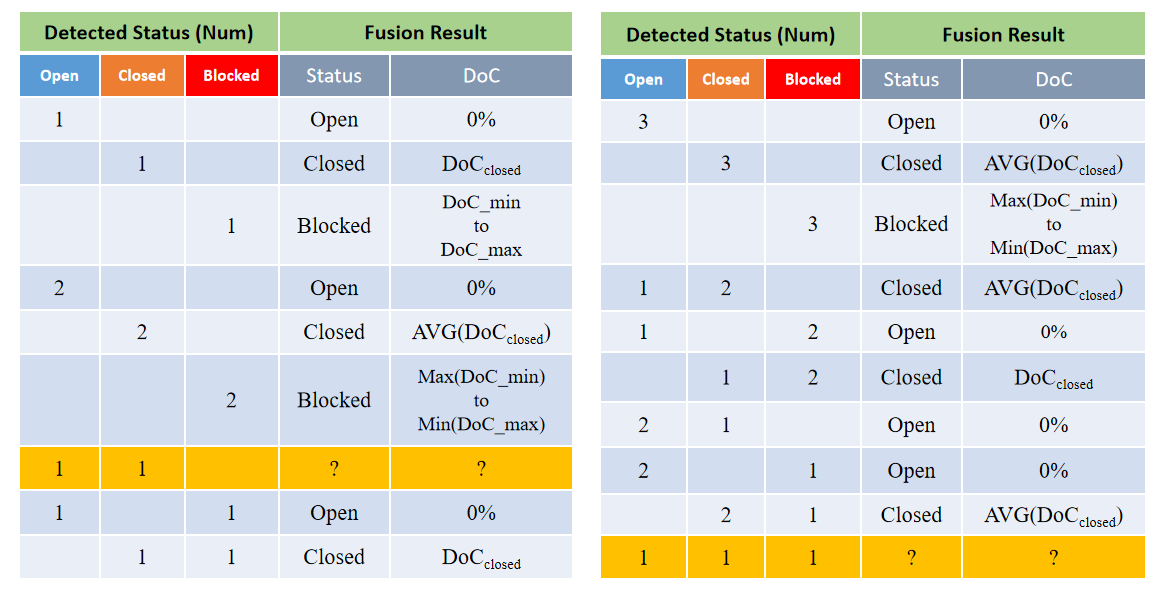
\includegraphics[width=0.9\textwidth]{Figures/Fusion Cases.png}
  \caption{All Detection Cases for up to three cameras and Pre-defined Fusion Results}
  \label{fig:13}  
\end{figure}

The 19 possible scenarios discussed earlier can be summarized and generalized, as shown in Figure \ref{fig:14}, based on the fusion results obtained through the pre-defined rules. However, in situations where the number of "open" and "closed" results are equal, it is difficult to determine the final status of the roller shutter accurately. Therefore, practice is needed before we make the decision.

\begin{figure}[h]
  \centering
  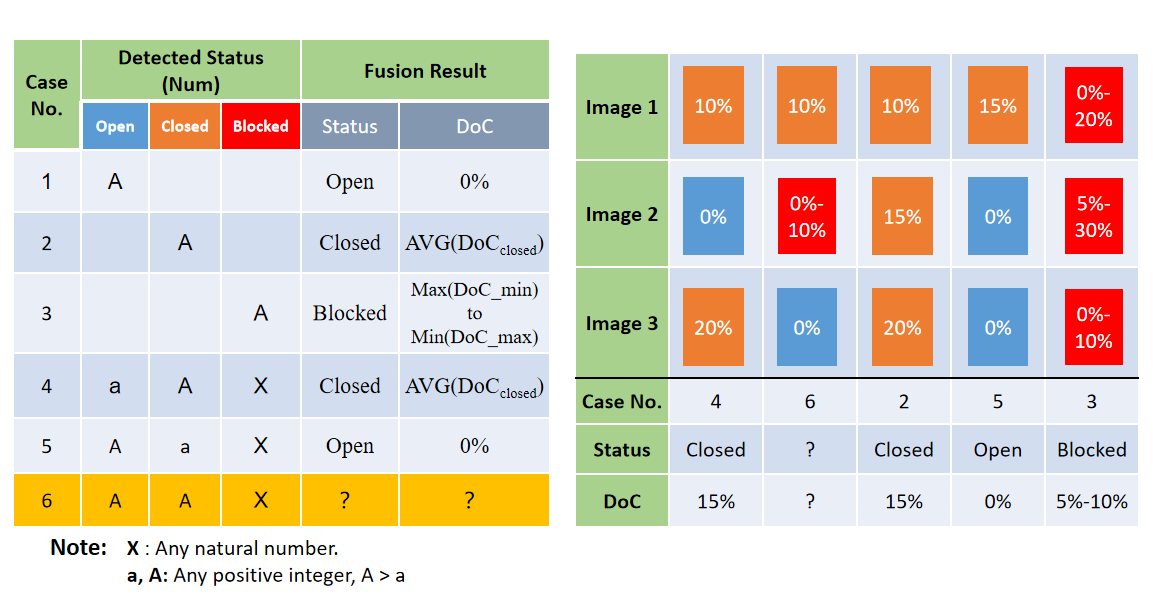
\includegraphics[width=0.9\textwidth]{Figures/Fusion.png}
  \caption{Fusion Logic Summary (Left) and an Example (Right) }
  \label{fig:14}  
\end{figure}
